% Working paper. Every result is a macro from numbers.tex or a table from tables/, written by
% code/06_paper_numbers.py from output/*.json. Build: pdflatex inspection_rd (twice).
\documentclass[11pt,letterpaper]{article}
\usepackage[T1]{fontenc}
\usepackage{charter}
\usepackage[margin=1in]{geometry}
\usepackage{setspace,amsmath,amssymb,graphicx,booktabs,array,multirow,enumitem,xcolor,url}
\usepackage[font=small,labelfont=bf]{caption}
\usepackage[authoryear,round]{natbib}
\usepackage[hidelinks]{hyperref}
\newcommand{\absentLater}{87}
\newcommand{\balMonthEighty}{+0.13}
\newcommand{\balMonthNinety}{+0.06}
\newcommand{\balMonthPEighty}{0.31}
\newcommand{\balMonthPNinety}{0.58}
\newcommand{\balMonthSeEighty}{0.13}
\newcommand{\balMonthSeNinety}{0.11}
\newcommand{\balPrevEighty}{$-$0.63}
\newcommand{\balPrevNinety}{+0.57}
\newcommand{\balPrevPEighty}{0.38}
\newcommand{\balPrevPNinety}{0.35}
\newcommand{\balPrevSeEighty}{0.72}
\newcommand{\balPrevSeNinety}{0.61}
\newcommand{\balSeqEighty}{$-$0.04}
\newcommand{\balSeqNinety}{$-$0.01}
\newcommand{\balSeqPEighty}{0.33}
\newcommand{\balSeqPNinety}{0.83}
\newcommand{\balSeqSeEighty}{0.04}
\newcommand{\balSeqSeNinety}{0.03}
\newcommand{\balYearEighty}{$-$0.03}
\newcommand{\balYearNinety}{+0.04}
\newcommand{\balYearPEighty}{0.64}
\newcommand{\balYearPNinety}{0.39}
\newcommand{\balYearSeEighty}{0.05}
\newcommand{\balYearSeNinety}{0.05}
\newcommand{\ciHiEighty}{0.47}
\newcommand{\ciHiNinety}{0.56}
\newcommand{\ciLoEighty}{$-$1.80}
\newcommand{\ciLoNinety}{$-$1.23}
\newcommand{\ciLoSdEighty}{0.13}
\newcommand{\ciLoSdNinety}{0.09}
\newcommand{\densLrEighty}{+0.056}
\newcommand{\densLrNinety}{+0.001}
\newcommand{\densZEighty}{+1.53}
\newcommand{\densZNinety}{+0.04}
\newcommand{\difMf}{12}
\newcommand{\difPHolmMf}{0.95}
\newcommand{\difPHolmPh}{0.95}
\newcommand{\difPMf}{0.92}
\newcommand{\difPPh}{0.48}
\newcommand{\difPh}{50}
\newcommand{\difSeMf}{112}
\newcommand{\difSePh}{70}
\newcommand{\difZMf}{+0.10}
\newcommand{\difZPh}{+0.71}
\newcommand{\excMf}{328}
\newcommand{\excPh}{273}
\newcommand{\excRatioMf}{7.0}
\newcommand{\excRatioPh}{10.1}
\newcommand{\excSeMf}{20}
\newcommand{\excSePh}{19}
\newcommand{\fsEighty}{1.08}
\newcommand{\fsNinety}{0.99}
\newcommand{\fsSeEighty}{0.024}
\newcommand{\fsSeNinety}{0.022}
\newcommand{\histDensLr}{+0.202}
\newcommand{\histDensPct}{22}
\newcommand{\histDensZ}{+3.14}
\newcommand{\jumpEighty}{$-$0.66}
\newcommand{\jumpNinety}{$-$0.33}
\newcommand{\leeCiHiEighty}{1.24}
\newcommand{\leeCiHiNinety}{1.30}
\newcommand{\leeCiLoEighty}{$-$3.33}
\newcommand{\leeCiLoNinety}{$-$2.70}
\newcommand{\leeHiEighty}{+0.10}
\newcommand{\leeHiNinety}{+0.40}
\newcommand{\leeLoEighty}{$-$2.28}
\newcommand{\leeLoNinety}{$-$1.88}
\newcommand{\leftLimitEighty}{81.0}
\newcommand{\leftLimitNinety}{83.8}
\newcommand{\mdeEighty}{1.5}
\newcommand{\mdeNinety}{1.4}
\newcommand{\misMf}{316}
\newcommand{\misPh}{223}
\newcommand{\misSeMf}{103}
\newcommand{\misSePh}{63}
\newcommand{\nEighty}{10,993}
\newcommand{\nIndex}{54,915}
\newcommand{\nIndexProps}{28,936}
\newcommand{\nNinety}{15,183}
\newcommand{\pEighty}{0.253}
\newcommand{\pHolmEighty}{0.505}
\newcommand{\pHolmNinety}{0.505}
\newcommand{\pNinety}{0.468}
\newcommand{\placEightyFour}{$-$0.27}
\newcommand{\placNinetyFour}{+0.02}
\newcommand{\placPEightyFour}{0.65}
\newcommand{\placPNinetyFour}{0.97}
\newcommand{\placPSeventyFour}{0.82}
\newcommand{\placSeEightyFour}{0.60}
\newcommand{\placSeNinetyFour}{0.47}
\newcommand{\placSeSeventyFour}{0.72}
\newcommand{\placSeventyFour}{$-$0.16}
\newcommand{\rddPEighty}{0.019}
\newcommand{\rddPNinety}{0.674}
\newcommand{\rddTEighty}{+2.34}
\newcommand{\rddTNinety}{$-$0.42}
\newcommand{\rdrBcEighty}{$-$0.10}
\newcommand{\rdrBcNinety}{$-$0.02}
\newcommand{\rdrConvEighty}{$-$0.36}
\newcommand{\rdrConvNinety}{$-$0.18}
\newcommand{\rdrHEighty}{3.69}
\newcommand{\rdrHNinety}{3.36}
\newcommand{\rdrHiEighty}{1.42}
\newcommand{\rdrHiNinety}{1.25}
\newcommand{\rdrLoEighty}{$-$1.62}
\newcommand{\rdrLoNinety}{$-$1.28}
\newcommand{\rdrPEighty}{0.895}
\newcommand{\rdrPNinety}{0.977}
\newcommand{\residSd}{13.5}
\newcommand{\robDonutHalfCiHiEighty}{0.48}
\newcommand{\robDonutHalfCiHiNinety}{0.84}
\newcommand{\robDonutHalfCiLoEighty}{$-$2.39}
\newcommand{\robDonutHalfCiLoNinety}{$-$1.48}
\newcommand{\robDonutHalfEighty}{$-$0.96}
\newcommand{\robDonutHalfNinety}{$-$0.32}
\newcommand{\robDonutHalfPEighty}{0.191}
\newcommand{\robDonutHalfPNinety}{0.594}
\newcommand{\robDonutHalfSeEighty}{0.73}
\newcommand{\robDonutHalfSeNinety}{0.59}
\newcommand{\robDonutOneCiHiEighty}{0.32}
\newcommand{\robDonutOneCiHiNinety}{1.32}
\newcommand{\robDonutOneCiLoEighty}{$-$3.44}
\newcommand{\robDonutOneCiLoNinety}{$-$1.75}
\newcommand{\robDonutOneEighty}{$-$1.56}
\newcommand{\robDonutOneNinety}{$-$0.22}
\newcommand{\robDonutOnePEighty}{0.104}
\newcommand{\robDonutOnePNinety}{0.784}
\newcommand{\robDonutOneSeEighty}{0.96}
\newcommand{\robDonutOneSeNinety}{0.78}
\newcommand{\robHEightCiHiEighty}{$-$0.46}
\newcommand{\robHEightCiHiNinety}{$-$0.01}
\newcommand{\robHEightCiLoEighty}{$-$2.27}
\newcommand{\robHEightCiLoNinety}{$-$1.44}
\newcommand{\robHEightEighty}{$-$1.37}
\newcommand{\robHEightNinety}{$-$0.72}
\newcommand{\robHEightPEighty}{0.003}
\newcommand{\robHEightPNinety}{0.048}
\newcommand{\robHEightSeEighty}{0.46}
\newcommand{\robHEightSeNinety}{0.37}
\newcommand{\robHThreeCiHiEighty}{1.22}
\newcommand{\robHThreeCiHiNinety}{0.96}
\newcommand{\robHThreeCiLoEighty}{$-$1.72}
\newcommand{\robHThreeCiLoNinety}{$-$1.32}
\newcommand{\robHThreeEighty}{$-$0.25}
\newcommand{\robHThreeNinety}{$-$0.18}
\newcommand{\robHThreePEighty}{0.738}
\newcommand{\robHThreePNinety}{0.760}
\newcommand{\robHThreeSeEighty}{0.75}
\newcommand{\robHThreeSeNinety}{0.58}
\newcommand{\robNotFirstCiHiEighty}{0.80}
\newcommand{\robNotFirstCiHiNinety}{0.58}
\newcommand{\robNotFirstCiLoEighty}{$-$2.04}
\newcommand{\robNotFirstCiLoNinety}{$-$1.88}
\newcommand{\robNotFirstEighty}{$-$0.62}
\newcommand{\robNotFirstNinety}{$-$0.65}
\newcommand{\robNotFirstPEighty}{0.392}
\newcommand{\robNotFirstPNinety}{0.301}
\newcommand{\robNotFirstSeEighty}{0.72}
\newcommand{\robNotFirstSeNinety}{0.63}
\newcommand{\robQuadCiHiEighty}{1.18}
\newcommand{\robQuadCiHiNinety}{0.82}
\newcommand{\robQuadCiLoEighty}{$-$1.45}
\newcommand{\robQuadCiLoNinety}{$-$1.25}
\newcommand{\robQuadEighty}{$-$0.13}
\newcommand{\robQuadNinety}{$-$0.21}
\newcommand{\robQuadPEighty}{0.843}
\newcommand{\robQuadPNinety}{0.684}
\newcommand{\robQuadSeEighty}{0.67}
\newcommand{\robQuadSeNinety}{0.53}
\newcommand{\seEighty}{0.58}
\newcommand{\seNinety}{0.46}
\newcommand{\secAttrEighty}{$-$3.5}
\newcommand{\secAttrNinety}{$-$4.0}
\newcommand{\secAttrPEighty}{0.000}
\newcommand{\secAttrPNinety}{0.000}
\newcommand{\secAttrSeEighty}{1.0}
\newcommand{\secAttrSeNinety}{1.0}
\newcommand{\secFailEighty}{+2.1}
\newcommand{\secFailNinety}{+0.5}
\newcommand{\secFailPEighty}{0.063}
\newcommand{\secFailPNinety}{0.535}
\newcommand{\secFailSeEighty}{1.1}
\newcommand{\secFailSeNinety}{0.8}
\newcommand{\secFixedEighty}{+0.50}
\newcommand{\secFixedNinety}{$-$0.36}
\newcommand{\secFixedPEighty}{0.412}
\newcommand{\secFixedPNinety}{0.425}
\newcommand{\secFixedSeEighty}{0.61}
\newcommand{\secFixedSeNinety}{0.46}
\newcommand{\shareNext}{91.6}
\newcommand{\thrMfEightyAbove}{8}
\newcommand{\thrMfEightyBelow}{$-$11}
\newcommand{\thrMfNinetyAbove}{5}
\newcommand{\thrMfNinetyBelow}{6}
\newcommand{\thrMfSixtyAbove}{17}
\newcommand{\thrMfSixtyBelow}{$-$30}
\newcommand{\thrPhEightyAbove}{10}
\newcommand{\thrPhEightyBelow}{$-$11}
\newcommand{\thrPhNinetyAbove}{11}
\newcommand{\thrPhNinetyBelow}{$-$1}
\newcommand{\thrPhSixtyAbove}{7}
\newcommand{\thrPhSixtyBelow}{$-$7}
\newcommand{\trimEighty}{3.6}
\newcommand{\trimNinety}{4.3}
\newcommand{\upcsDifMf}{1,160}
\newcommand{\upcsDifPh}{464}
\newcommand{\upcsDifSeMf}{263}
\newcommand{\upcsDifSePh}{146}
\newcommand{\upcsExcMf}{-22}
\newcommand{\upcsExcPh}{13}
\newcommand{\upcsExcSeMf}{23}
\newcommand{\upcsExcSePh}{16}
\newcommand{\upcsMisMf}{-1,182}
\newcommand{\upcsMisPh}{-451}
\newcommand{\waldEighty}{$-$0.61}
\newcommand{\waldNinety}{$-$0.33}
\newcommand{\waldSeEighty}{0.54}
\newcommand{\waldSeNinety}{0.46}

\onehalfspacing
\setlist{itemsep=0.2ex,topsep=0.4ex}
\newcommand{\col}[1]{\texttt{\small #1}}
\sloppy

\title{Do Inspection Thresholds Improve Housing Conditions?\\[0.3ex]\large Regression Discontinuity Evidence from HUD's Physical Inspection Schedule}
\author{Ayishatu Ameen\thanks{Independent Researcher, Hartford, Connecticut, USA. E-mail: ameenayishatu4@gmail.com. ORCID: 0009-0009-9386-2526. The pre-analysis plan is registered at \url{https://osf.io/ab2es}. Data: \url{https://doi.org/10.5281/zenodo.23200319}. Code and outputs: \url{https://github.com/AYISHATUAMEEN/inspection-rd}. Code and drafts were prepared with the assistance of Claude (Anthropic); the author made the analytic decisions, registered the plan, and is responsible for all content. No external funding; no competing interests.}}
\date{October 2026\\[0.5ex]\small Working paper. Comments welcome.}

\begin{document}
\maketitle
\begin{abstract}
\noindent HUD inspects assisted multifamily properties every three years if they score 90 or above, every two years if they score 80 to 89, and every year if they score below 80. I use these cutoffs in a pre-registered regression discontinuity design to ask whether a longer interval between inspections lowers a property's score at its next inspection. Among \nIndex{} inspections conducted between 2001 and 2005, crossing a cutoff lengthens the interval to the next inspection by about a year, but the next score changes by \jumpEighty{} points (95\% CI \ciLoEighty{} to \ciHiEighty) at 80 and \jumpNinety{} points (\ciLoNinety{} to \ciHiNinety) at 90. Both estimates are small and statistically indistinguishable from zero, and the result is robust to bandwidth choice, bias-corrected inference, donut specifications and bounds for differential attrition. The primary estimates rule out declines larger than about 1.8 points at 80 and 1.2 points at 90; the donut estimate at 80, the registered headline there because of evidence of sorting, is less precise. A second registered analysis examines the excess of scores at exactly 59 under the National Standards for the Physical Inspection of Real Estate (NSPIRE). The excess (\excMf{} multifamily and \excPh{} public housing inspections) matches the mass missing from scores 60 to 70, as the unit-threshold scoring rule predicts if it alone produces the excess. Under the earlier protocol, by contrast, scores show sorting just above the passing score and the 80 cutoff. A third registered analysis of HUD's decision to begin scoring affirmative requirements on 1~October 2026 awaits data.
\end{abstract}

\noindent\textbf{JEL codes:} R38, H83, K23, I18, C21.\\
\textbf{Keywords:} housing inspection, regulatory monitoring, regression discontinuity, bunching, assisted housing, NSPIRE, pre-registration.

\section{Introduction}
Regulators who cannot watch everyone ration their attention by risk. A firm, a restaurant or a landlord that scored well last time is inspected less often next time. The design is efficient if conditions do not slip while the regulator is away, and self-defeating if they do. Whether monitoring frequency itself changes compliance is therefore a central question for the design of inspection regimes, and one the empirical literature has addressed mostly for workplaces, restaurants and polluters \citep{jin2003, levine2012, duflo2013, gray2011}.

Housing that the federal government subsidizes is inspected under exactly this kind of rule. Since 2001, the U.S. Department of Housing and Urban Development (HUD) has set the inspection interval of each assisted multifamily property from its previous score: properties scoring 90 or above are inspected once every three years, those scoring 80 to 89 every two years, and those below 80 every year \citep{fr2000}. The rule creates two sharp changes in monitoring intensity at arbitrary points of a continuous score. Two properties scoring 79.4 and 79.5 are, to a first approximation, in the same condition; one will be inspected again in a year and the other in two.

I exploit these cutoffs in a regression discontinuity (RD) design. The analysis was registered before any outcome was examined \citep{osfplan}. Using HUD's history file of multifamily inspections, I compare properties just above and just below each cutoff in their score at the next inspection. The first stage is strong: crossing either cutoff lengthens the interval to the next inspection by about one year, almost exactly as the rule prescribes. The reduced form is not. At the 80 cutoff the next score is \jumpEighty{} points lower just above the cutoff (standard error \seEighty); at the 90 cutoff, \jumpNinety{} (\seNinety). Neither is statistically significant, and the confidence intervals exclude declines larger than \ciLoSdEighty{} and \ciLoSdNinety{} residual standard deviations. The pattern holds across bandwidths, with bias-corrected inference, when observations closest to the cutoff are dropped, and within bounds for the differential attrition that a longer interval mechanically induces.

The second question concerns the current protocol. Under NSPIRE, which replaced the earlier Uniform Physical Condition Standards (UPCS) in 2023, \citet{ameen2026} documents that 2.3\% of all scores are exactly 59, one point below the pass mark. HUD's scoring notice assigns 59 to any property whose unit deficiencies account for 30 or more points of deductions, whatever its total \citep{nspirescoring}. Because such a property's score cannot exceed 70, the rule can only move mass to 59 from the range 60 to 70. A purely mechanical account therefore makes a sharp prediction: the excess at 59 equals the deficit between 60 and 70. The registered bunching analysis finds exactly that, for both multifamily and public housing. The earlier protocol, which had no such rule, shows a different signature: fewer scores than expected just below 60 and 80 and more just above, the pattern one would expect when owners contest scores that fall just short of a threshold and the regulations reward a successful challenge that moves a property across it \citep{fr2000}.

The third question, registered in advance and not yet answerable, concerns HUD's decision to include deficiencies under NSPIRE's new affirmative requirements in scores from 1~October 2026 \citep{fr2026}. Section~\ref{sec:h3} states the design that will be applied when HUD publishes the first file covering inspections after that date.

The paper contributes to three literatures. First, to the economics of monitoring and enforcement \citep{gray2011, shimshack2014}, it adds a quasi-experimental estimate of the effect of inspection frequency in a setting, housing, where the outcome is the regulator's own measure of condition. Second, to the RD literature on administrative thresholds \citep{lee2010}, it contributes an application where the running variable is itself the object of strategic behaviour in one regime but not the other, and documents how that difference appears in the data. Third, to research on assisted housing quality \citep{gao2019}, it offers evidence that, near the thresholds, the schedule's longer intervals did not measurably erode the condition HUD observes next.

\section{Institutional Background}\label{sec:background}
\subsection{Inspections and the score}
HUD's Real Estate Assessment Center inspects public housing and HUD-assisted or HUD-insured multifamily properties. Under UPCS, in force for multifamily properties until 1~October 2023, an inspector examined the site, building exteriors, building systems, common areas and a sample of units, recorded deficiencies by severity, and the scoring model converted them to a score out of 100 \citep{fr2000}. Scores below 60 fail and trigger enforcement steps; properties scoring 30 or below are referred to HUD's Departmental Enforcement Center.

\subsection{The inspection schedule}
24 CFR 200.857(b), effective 8 January 2001, designates a property scoring 90 or higher a ``standard 1'' property, inspected once every three years; a property scoring at least 80 but less than 90 a ``standard 2'' property, inspected every two years; and a property scoring below 80 a ``standard 3'' property, inspected annually \citep{fr2000}. Scores may include fractions. For designation they are rounded to the nearest whole point, with halves rounded up (89.5 becomes 90), so the operative cutoffs on the unrounded score are 79.5 and 89.5. The regulation also permits owners to request a technical review of a score when correcting an objectively verifiable error would ``significantly improve'' it, defined as moving the property across a threshold or raising its score by ten points or more. Public housing adopted a similar project-level schedule only with the 2011 interim rule of the Public Housing Assessment System, with exceptions for small agencies and agencies designated troubled; I therefore restrict the main analysis to multifamily properties.

\subsection{NSPIRE, the score of 59, and the 2026 change}
NSPIRE took effect on 1~July 2023 for public housing and 1~October 2023 for multifamily programs \citep{nspirerule}. It keeps the 0--100 scale, the passing score of 60 and the 3-2-1 schedule \citep{cfr5705}, but changes how deficiencies are counted and weighted. Its scoring notice adds a unit threshold: if deductions from deficiencies inside units total 30 points or more, the property fails with a score of 59, whatever its total score \citep{nspirescoring}. NSPIRE also introduced affirmative requirements (for example GFCI protection, guardrails, interior lighting and minimum electrical standards). Deficiencies under them were recorded but not scored for an initial period that HUD extended twice; HUD's notice of 29 September 2026 confirms that from 1~October 2026 they enter the score \citep{fr2026}.

\section{Data}\label{sec:data}
The data are the Assisted Housing Condition Panel (AHCP) v1.0 \citep{ahcp, ameen2026}, which reconstructs inspection histories from the nine physical inspection score files HUD still publishes. For the RD analysis I use HUD's 2011 history file, which lists up to ten multifamily inspections per property for 2000 to 2009, with scores reported to two decimals. Later files list only each property's latest inspection and report integer scores, so they cannot supply the next inspection reliably.

An \emph{index inspection} is a multifamily inspection dated between 8~January 2001, when the schedule took effect, and 31~December 2005, which leaves at least 46 months for the next inspection to be observed before the file ends in November 2009. There are \nIndex{} index inspections of \nIndexProps{} properties; \shareNext\% have a later inspection listed. The outcome is the score at that next inspection. Table~\ref{tab:summary} describes the sample.

\begin{table}[t]
\centering\small
\caption{Primary sample: multifamily index inspections, 2001--2005}\label{tab:summary}
\begin{tabular}{lrrrrr}
\toprule
Variable & $n$ & Mean & SD & P10 & P90 \\
\midrule
Index score & 54,915 & 81.80 & 15.05 & 61.08 & 97.74 \\
Next score & 50,317 & 81.10 & 14.98 & 60.58 & 97.03 \\
Years to next inspection & 50,317 & 2.37 & 1.14 & 0.94 & 3.94 \\
Previous score (where listed) & 32,474 & 76.47 & 15.61 & 55.39 & 95.35 \\
Inspection year & 54,915 & 2002.78 & 1.34 & 2001.00 & 2005.00 \\
Share below 60 at index & 54,915 & 8.7\% & & & \\
Share 80 or above at index & 54,915 & 64.1\% & & & \\
Share 90 or above at index & 54,915 & 38.3\% & & & \\
\bottomrule
\end{tabular}

\par\vspace{0.5ex}\footnotesize\raggedright Notes: Index inspections from HUD's 2011 history file. ``Next'' variables are for index inspections with a later inspection listed. P10 and P90 are the 10th and 90th percentiles.
\end{table}

For the bunching analyses I use all AHCP inspections flagged NSPIRE (multifamily and public housing separately) and, for comparison, all UPCS inspections dated 2013 to 2019, which carry integer scores.

\section{Empirical Strategy}\label{sec:strategy}
\subsection{Design and estimand}
Let $x_i$ be the index score of inspection $i$, $c\in\{79.5, 89.5\}$ a cutoff, $D_i=\mathbb{1}[x_i\ge c]$, and $y_i$ the score at the property's next inspection. The registered primary estimate is the jump $\tau$ in a local linear regression on each side of the cutoff,
\begin{equation}
y_i=\alpha+\tau D_i+\beta(x_i-c)+\gamma D_i(x_i-c)+\varepsilon_i,\qquad |x_i-c|\le h,
\end{equation}
with a triangular kernel, a fixed bandwidth of $h=5$ score points, and standard errors clustered by property. The bandwidth was fixed in the plan so that no tuning choice depends on the outcome, and it keeps each window clear of the other cutoff. H1a and H1b (the 80 and 90 cutoffs) are tested two-sided at the 5\% level, with Holm's correction across the two.

The estimand is the effect of being \emph{assigned} the longer interval on the score the regulator observes at its next visit. Because that visit occurs about a year later on the longer-interval side, the estimand combines any effect of reduced monitoring with an extra year of elapsed time. A registered secondary outcome holds elapsed time roughly fixed: the score at the first inspection at least 21 months after the index inspection. Dividing $\tau$ by the first-stage jump in the interval gives a fuzzy estimate per additional year.

\subsection{Identifying assumption and threats}
The design requires that properties just above and below a cutoff would have had the same expected next score under the same schedule. Three threats are pre-specified. \emph{Sorting}: if owners or inspectors push scores across a cutoff, properties just above it may differ. I test the density of the running variable \citep{mccrary2008, cattaneo2020} and, as registered, make a donut estimate excluding scores within one point of the cutoff the headline if the density test rejects. \emph{Differential attrition}: a property assigned a longer interval has an extra year in which to leave HUD's portfolio before its next inspection, so its outcome is less often observed. I report trimming bounds \citep{lee2009}. \emph{Imbalance}: I test four predetermined variables (previous score, inspection sequence number, index year and month).

\section{Results}\label{sec:results}
\subsection{First stage}
Figure~\ref{fig:firststage} shows the mean interval to the next inspection by index score. The schedule is followed closely. Just below 80, properties are reinspected after \leftLimitEighty{} years on average; crossing the cutoff adds \fsEighty{} years (standard error \fsSeEighty). Just below 90 the interval is \leftLimitNinety{} years and crossing adds \fsNinety{} (\fsSeNinety). The design is close to sharp.

\begin{figure}[t]
\centering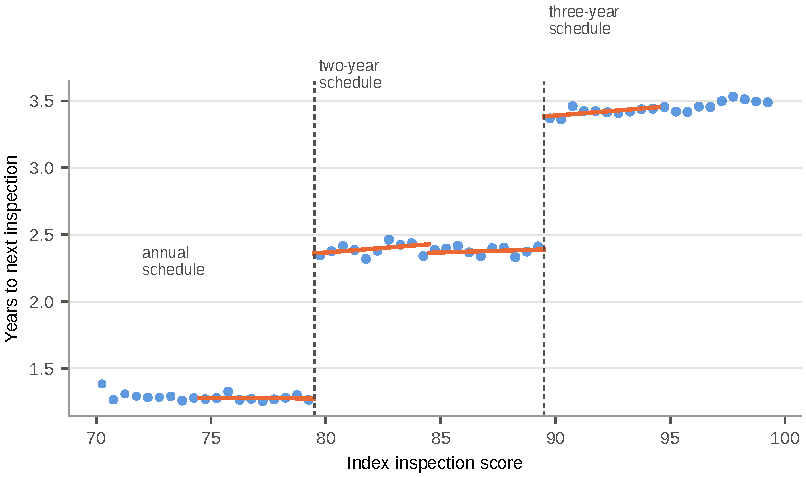
\includegraphics[width=0.92\textwidth]{figs/first_stage.pdf}
\caption{First stage: years to the next inspection by index score. Dots are means in half-point bins (size proportional to count); lines are local linear fits within five points of each cutoff. Dashed lines mark the cutoffs at 79.5 and 89.5.}\label{fig:firststage}
\end{figure}

\subsection{Validity}
\emph{Density.} Figure~\ref{fig:density} shows the distribution of index scores. At 90 there is no sign of sorting (\texttt{rddensity} $t=\rddTNinety$, $p=\rddPNinety$). At 80 the evidence is mixed: the registered binned estimator gives a log density ratio of \densLrEighty{} ($z=\densZEighty$), while \texttt{rddensity} rejects continuity ($t=\rddTEighty$, $p=\rddPEighty$). The plan named both tests without saying which governs the decision rule. I apply the stricter reading and treat the 80 cutoff as showing sorting; the donut estimate is therefore the headline at 80 (Section~\ref{sec:main}). The sorting is not surprising: Section~\ref{sec:bunching} shows a similar pattern at 80 in later data, and the technical-review rule rewards challenges that move a property across a threshold.

\begin{figure}[t]
\centering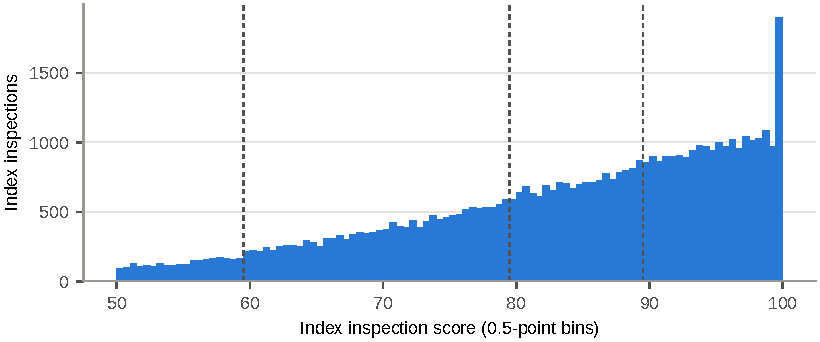
\includegraphics[width=0.92\textwidth]{figs/density.pdf}
\caption{Distribution of index inspection scores, 2001--2005, half-point bins. Dashed lines mark 59.5, 79.5 and 89.5.}\label{fig:density}
\end{figure}

\emph{Balance.} None of the four predetermined variables jumps at either cutoff. The previous score differs by \balPrevEighty{} points (\balPrevSeEighty; $p=\balPrevPEighty$) at 80 and \balPrevNinety{} (\balPrevSeNinety; $p=\balPrevPNinety$) at 90; inspection sequence, year and month show no discontinuity either (all $p\ge0.31$; see the output files).

\emph{Attrition.} The share of index inspections with a next inspection listed changes by \secAttrEighty{} percentage points at 80 (standard error \secAttrSeEighty) and \secAttrNinety{} at 90 (\secAttrSeNinety). \absentLater\% of index inspections without a next inspection belong to properties absent from every later HUD file, consistent with exit from the portfolio during the extra year.

\subsection{Main results}\label{sec:main}
Figure~\ref{fig:rf} plots the next score against the index score, and Table~\ref{tab:rd} reports the estimates. The registered primary estimates are \jumpEighty{} points at 80 (standard error \seEighty; 95\% CI \ciLoEighty{} to \ciHiEighty; $p=\pEighty$, Holm $p=\pHolmEighty$) and \jumpNinety{} at 90 (\seNinety; \ciLoNinety{} to \ciHiNinety; $p=\pNinety$, Holm $p=\pHolmNinety$). Neither null hypothesis is rejected. The fuzzy estimates are \waldEighty{} (\waldSeEighty) and \waldNinety{} (\waldSeNinety) points per additional year between inspections.

\begin{figure}[t]
\centering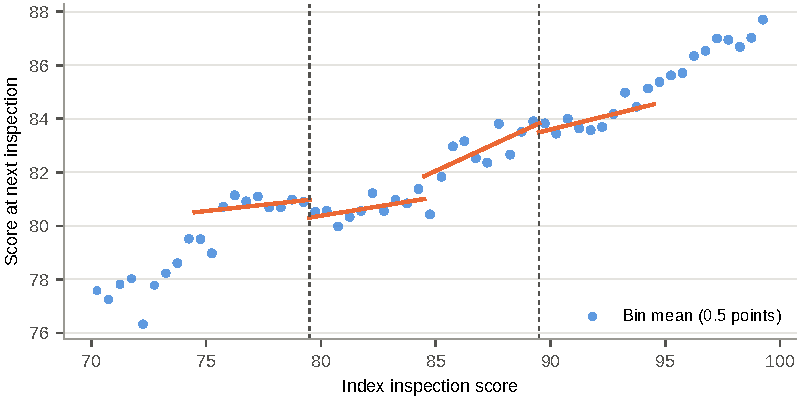
\includegraphics[width=0.92\textwidth]{figs/reduced_form.pdf}
\caption{Reduced form: score at the next inspection by index score. Dots are means in half-point bins; lines are local linear fits within five points of each cutoff.}\label{fig:rf}
\end{figure}

\begin{table}[t]
\centering\small
\caption{Effect of crossing an inspection-schedule cutoff on the next score}\label{tab:rd}
\begin{tabular}{lcc}
\toprule
& 80 cutoff & 90 cutoff \\
\midrule
Primary: local linear, $h=5$ & $-$0.66 & $-$0.33 \\
 & (0.58) & (0.46) \\
Bandwidth $h=3$ & $-$0.25 & $-$0.18 \\
 & (0.75) & (0.58) \\
Bandwidth $h=8$ & $-$1.37 & $-$0.72 \\
 & (0.46) & (0.37) \\
Local quadratic, $h=8$ & $-$0.13 & $-$0.21 \\
 & (0.67) & (0.53) \\
Donut, $|x-c|\geq0.5$ & $-$0.96 & $-$0.32 \\
 & (0.73) & (0.59) \\
Donut, $|x-c|\geq1$ & $-$1.56 & $-$0.22 \\
 & (0.96) & (0.78) \\
Excluding first listed inspection & $-$0.62 & $-$0.65 \\
 & (0.72) & (0.63) \\
\texttt{rdrobust}, bias-corrected & $-$0.10 & $-$0.02 \\
\quad robust 95\% CI; MSE-optimal $h$ & [$-$1.62, 1.42]; 3.69 & [$-$1.28, 1.25]; 3.36 \\
Trimming bounds (attrition) & [$-$2.28, +0.10] & [$-$1.88, +0.40] \\
\midrule
Observations, primary & 10,993 & 15,183 \\
First stage (years), primary & 1.08 (0.024) & 0.99 (0.022) \\
\bottomrule
\end{tabular}

\par\vspace{0.5ex}\footnotesize\raggedright Notes: Each cell is the jump in the next inspection score at the cutoff, in points, from a local linear regression with a triangular kernel unless stated, with standard errors clustered by property in parentheses. \texttt{rdrobust} uses the MSE-optimal bandwidth and robust bias-corrected inference \citep{calonico2014}. Trimming bounds follow \citet{lee2009}, trimming the below-cutoff outcomes by the excess follow-up share.
\end{table}

Because the density test rejects at 80 under the stricter reading, the registered headline there is the donut estimate excluding scores within one point of the cutoff: \robDonutOneEighty{} (\robDonutOneSeEighty; $p=\robDonutOnePEighty$). It is larger in magnitude than the primary estimate and less precise (95\% CI \robDonutOneCiLoEighty{} to \robDonutOneCiHiEighty), and also not significant.

\subsection{Robustness}
Figure~\ref{fig:robust} and Table~\ref{tab:rd} collect the registered robustness checks. With the MSE-optimal bandwidth (\rdrHEighty{} and \rdrHNinety{} points) and robust bias-corrected confidence intervals, the estimates are \rdrBcEighty{} (\rdrLoEighty{} to \rdrHiEighty) and \rdrBcNinety{} (\rdrLoNinety{} to \rdrHiNinety). The trimming bounds are [\leeLoEighty, \leeHiEighty] at 80 and [\leeLoNinety, \leeHiNinety] at 90, and both include zero. Placebo cutoffs at 74.5, 84.5 and 94.5 show no jump ($p=\placPSeventyFour$, \placPEightyFour, \placPNinetyFour).

One pattern deserves comment. With a wider bandwidth of eight points, the local linear estimates become larger and significant (\robHEightEighty, $p=\robHEightPEighty$, at 80; \robHEightNinety, $p=\robHEightPNinety$, at 90). Allowing curvature at the same bandwidth removes them (\robQuadEighty{} and \robQuadNinety). Figure~\ref{fig:rf} shows why: the relation between index and next score is concave within each schedule band, so a straight line fitted over eight points on each side misplaces the limits. I read the wide-bandwidth linear estimates as specification error rather than evidence of an effect; the data-driven bandwidths, which balance bias and variance, are narrower than the primary five points.

\begin{figure}[t]
\centering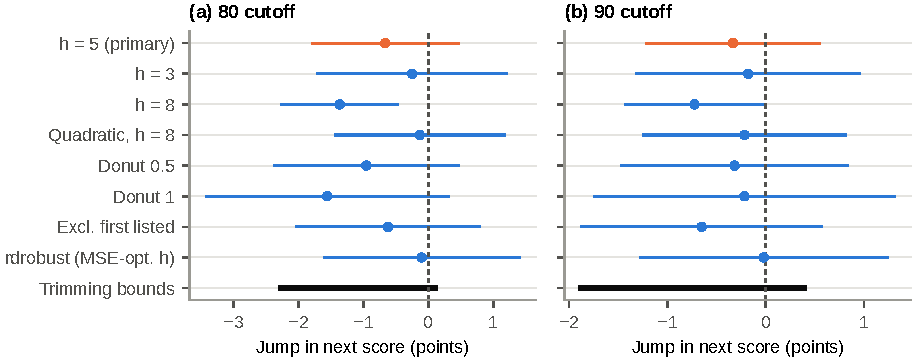
\includegraphics[width=0.92\textwidth]{figs/robustness.pdf}
\caption{Estimates across registered specifications with 95\% confidence intervals; the primary estimate is highlighted. The black bar is the trimming-bound interval for differential attrition.}\label{fig:robust}
\end{figure}

\subsection{Secondary outcomes}
The probability that the next inspection fails changes by \secFailEighty{} percentage points at 80 (\secFailSeEighty; $p=\secFailPEighty$) and \secFailNinety{} at 90 (\secFailSeNinety; $p=\secFailPNinety$). The fixed-horizon score, which compares properties at roughly the same elapsed time, changes by \secFixedEighty{} (\secFixedSeEighty) at 80 and \secFixedNinety{} (\secFixedSeNinety) at 90. None of these is significant, although the point estimate for failure at 80 is positive and its $p$-value is close to 0.06.

\section{Is the Mass at 59 Mechanical?}\label{sec:bunching}
Figure~\ref{fig:bunching} shows the distribution of NSPIRE scores with the counterfactual fitted to scores outside 55 to 72. The excess at 59 is \excMf{} inspections for multifamily (standard error \excSeMf) and \excPh{} for public housing (\excSePh), \excRatioMf{} and \excRatioPh{} times the counterfactual count. The mass missing from 60 to 70 is \misMf{} (\misSeMf) and \misPh{} (\misSePh). The registered test statistic, excess minus missing, is \difMf{} (\difSeMf; $z=\difZMf$, Holm $p=\difPHolmMf$) for multifamily and \difPh{} (\difSePh; $z=\difZPh$, Holm $p=\difPHolmPh$) for public housing. The excess at 59 is fully accounted for by the deficit just above it, as the unit-threshold rule predicts if it alone produces the excess.

\begin{figure}[t]
\centering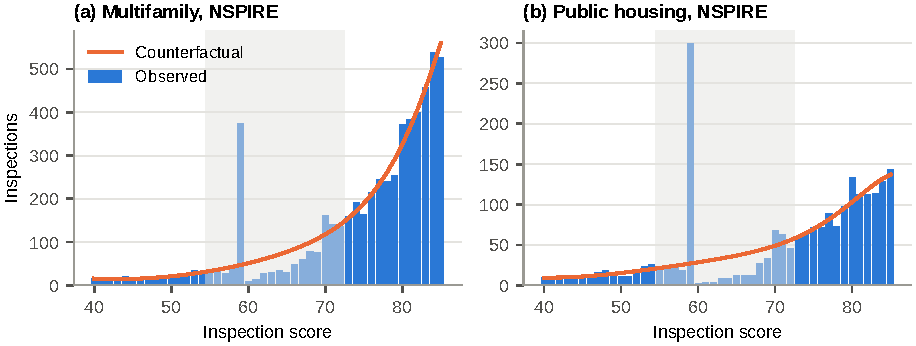
\includegraphics[width=0.95\textwidth]{figs/bunching.pdf}
\caption{NSPIRE scores and counterfactual distribution. Bars are observed counts at each integer score; the line is a fifth-order polynomial in log counts fitted outside the shaded range 55--72.}\label{fig:bunching}
\end{figure}

\begin{table}[t]
\centering\small
\caption{Excess mass at 59 and missing mass at 60--70}\label{tab:bunching}
\begin{tabular}{llcrrr}
\toprule
Sample & Order & Excluded & Excess at 59 & Missing in 60--70 & Difference \\
\midrule
Multifamily & 5 & 55--72 & 328 (20) & 316 (103) & 12 (112) \\
 & 4 & 55--72 & 328 (21) & 370 (157) & -42 (167) \\
 & 6 & 55--72 & 322 (27) & 428 (356) & -106 (375) \\
 & 5 & 53--74 & 336 (23) & 139 (151) & 197 (164) \\
 & 5 & 56--71 & 327 (21) & 318 (86) & 9 (94) \\
\quad UPCS 2013--19 (comparison) & 5 & 55--72 & -22 (23) & -1,182 (248) & 1,160 (263) \\
\midrule
Public housing & 5 & 55--72 & 273 (19) & 223 (63) & 50 (70) \\
 & 4 & 55--72 & 273 (18) & 250 (88) & 23 (94) \\
 & 6 & 55--72 & 271 (20) & 251 (229) & 20 (241) \\
 & 5 & 53--74 & 282 (18) & 111 (79) & 171 (86) \\
 & 5 & 56--71 & 275 (17) & 179 (50) & 97 (55) \\
\quad UPCS 2013--19 (comparison) & 5 & 55--72 & 13 (16) & -451 (136) & 464 (146) \\
\bottomrule
\end{tabular}

\par\vspace{0.5ex}\footnotesize\raggedright Notes: Counts of inspections relative to a polynomial counterfactual in log counts fitted to integer scores 40--85 outside the excluded range. Bootstrap standard errors (Poisson resampling of counts) in parentheses. The first row of each program is the registered specification.
\end{table}

Table~\ref{tab:bunching} shows how the result depends on the counterfactual. Polynomial order and a narrower excluded window leave it unchanged. A wider excluded window (53 to 74) leaves less data to anchor the curve near the threshold and produces a larger positive difference, significant at conventional levels for public housing. Two further caveats apply. The public files do not report unit deductions, so the rule's application cannot be observed directly; the finding is that the distribution is consistent with a purely mechanical account. And the same statistic computed on UPCS scores from 2013 to 2019, where no rule operates, correctly finds no excess at 59 (\upcsExcMf{} and \upcsExcPh) but a nonzero difference, because under UPCS the range 60 to 70 holds \emph{more} inspections than the counterfactual. That surplus is itself a sign of sorting, to which I now turn.

\subsection{Sorting at the thresholds under UPCS}
Table~\ref{tab:thresholds} compares observed and counterfactual counts at the two scores below and the two at or above each threshold, for UPCS inspections from 2013 to 2019. Multifamily scores show a large deficit just below 60 (\thrMfSixtyBelow\%) and a surplus just above (\thrMfSixtyAbove\%), and a smaller version of the same pattern at 80 (\thrMfEightyBelow\% and \thrMfEightyAbove\%). Public housing shows the pattern at 80 and, weakly, at 60. At 90 there is no clear asymmetry. The 2001 to 2005 history sample shows the same at 60: the density of index scores is about \histDensPct\% higher just above 59.5 than just below ($z=\histDensZ$). Movement from just below a threshold to just above it is what the technical-review rule rewards. Under NSPIRE, the corresponding range just above 60 is depleted rather than inflated, because the unit-threshold rule moves properties the other way.

\begin{table}[t]
\centering\small
\caption{Observed and counterfactual counts around thresholds, UPCS 2013--2019}\label{tab:thresholds}
\begin{tabular}{lrrrrrrr}
\toprule
& & \multicolumn{3}{c}{Two scores below} & \multicolumn{3}{c}{Two scores at or above} \\
\cmidrule(lr){3-5}\cmidrule(lr){6-8}
Program & Threshold & Observed & Counterf. & Diff. (\%) & Observed & Counterf. & Diff. (\%) \\
\midrule
Multifamily & 60 & 473 & 671 & $-$30 & 942 & 804 & 17 \\
 & 80 & 2,440 & 2,737 & $-$11 & 3,343 & 3,106 & 8 \\
 & 90 & 4,841 & 4,564 & 6 & 5,202 & 4,949 & 5 \\
Public housing & 60 & 266 & 285 & $-$7 & 347 & 323 & 7 \\
 & 80 & 736 & 827 & $-$11 & 999 & 908 & 10 \\
 & 90 & 1,226 & 1,245 & $-$1 & 1,444 & 1,299 & 11 \\
\bottomrule
\end{tabular}

\par\vspace{0.5ex}\footnotesize\raggedright Notes: Counterfactual counts from a quadratic in the score fitted to integer scores $c-10$ to $c+9$, excluding $c-2$ to $c+1$. Registered as descriptive; no standard errors were pre-specified.
\end{table}

\section{The October 2026 Change}\label{sec:h3}
From 1~October 2026, deficiencies under NSPIRE's affirmative requirements count toward the score \citep{fr2026}. The registered hypothesis is that, for the same properties, NSPIRE inspections on or after that date have lower scores, a higher share below 60 and a higher share at exactly 59. The analysis will be run once, on the first HUD file whose inspections reach at least 31~March 2027, by regressing each outcome on an indicator for inspection after the change with property fixed effects and program-by-year effects, clustering by property, with Holm's correction across the three outcomes. The plan states one limitation in advance: properties reinspected soon after the change are disproportionately those that scored low before, which biases a before-and-after comparison toward improvement, and the fixed effects do not remove this.

\section{Discussion}\label{sec:discussion}
\paragraph{What the null means.} Near the 80 and 90 thresholds, being assigned a longer interval between inspections did not measurably lower the score at the next inspection, even though the next visit came a year later. Three readings are consistent with this. Conditions may simply change slowly enough that an extra year makes little difference for properties that scored in the 75--95 range. Owners may maintain to a standard set by other pressures (lenders, local codes, residents) rather than by the federal inspection calendar. Or reduced monitoring may lower effort while the anticipated inspection still disciplines it, with effects too small to detect. The design cannot separate these. What it can say is that for properties near these thresholds, the primary estimates rule out declines in the next score larger than \ciLoEighty{} points at 80 and \ciLoNinety{} at 90 (about \ciLoSdEighty{} and \ciLoSdNinety{} residual standard deviations). The donut estimate at 80 is less precise and cannot exclude declines of up to \robDonutOneCiLoEighty{} points.

\paragraph{Scope.} The estimates apply to multifamily properties scoring near 80 and 90 in 2001 to 2005, under UPCS. They say nothing directly about low-scoring properties, which are inspected annually regardless, about public housing, or about NSPIRE, whose scoring places more weight on unit conditions. The outcome is HUD's own score, which measures what the protocol records and is itself subject to inspector variation \citep{gao2019}. The longer-interval side is observed after an extra year, and its outcome is less often observed; the fixed-horizon outcome and the trimming bounds address these but cannot eliminate them.

\paragraph{The scores as a measure.} The bunching results matter for anyone who uses these scores. Under UPCS, scores just below the passing mark and the 80 cutoff are under-represented, consistent with successful challenges by owners. Under NSPIRE, the excess at 59 reflects a rule, and a score of 59 is a category (``failed on unit conditions'') rather than a point on a continuous scale. Analyses that treat scores near 60 as continuous, including RD designs at the passing score, need to account for both.

\section{Conclusion}
HUD's inspection schedule assigns substantially different monitoring intensity to properties in nearly identical condition. A pre-registered RD analysis of that schedule finds no measurable effect of a longer interval on the next inspection score near the 80 and 90 thresholds, with confidence intervals that rule out large declines. The excess of NSPIRE scores at exactly 59 matches what the unit-threshold rule would produce on its own, while the earlier protocol shows sorting toward passing. The October 2026 change in what NSPIRE scores will be examined, as registered, when the data exist.

\section*{Deviations from the Pre-Analysis Plan}
\begin{enumerate}
\item \textbf{Density test at 80.} The plan named two density tests (a binned local linear estimator and \texttt{rddensity}) but did not say which governs the decision rule. They disagree at 80 ($z=\densZEighty$ versus $p=\rddPEighty$). I applied the stricter reading, so the donut estimate is the headline at 80. The primary estimate is reported alongside it.
\item \textbf{Software.} \texttt{rdrobust} 2.1.1 and \texttt{rddensity} 3.0 were installed from verified PyPI wheels. Their plotting dependency (\texttt{plotnine}) was replaced by an import-only stub because no plots from those packages are used. \texttt{rdrobust} detects mass points in the running variable (scores to two decimals contain ties) and applies its default adjustment.
\item \textbf{H3} has not been run because the data do not yet exist, as anticipated in the plan.
\end{enumerate}
No other departures. The confirmatory outputs were produced by the registered scripts without manual steps; the repository's commit history records that the code preceded the results.

\begin{thebibliography}{99}\small\setlength{\itemsep}{0.1ex}
\bibitem[Ameen(2026a)]{ahcp} Ameen, A. (2026a). \emph{Assisted Housing Condition Panel (AHCP) v1.0} [dataset]. Zenodo. doi:10.5281/zenodo.23200319.
\bibitem[Ameen(2026b)]{ameen2026} Ameen, A. (2026b). The Assisted Housing Condition Panel: reconstructing inspection histories for HUD-assisted housing from overwritten public score files. Working paper.
\bibitem[Ameen(2026c)]{osfplan} Ameen, A. (2026c). Do inspection thresholds improve housing conditions? Pre-analysis plan. OSF Registries. \url{https://osf.io/ab2es}.
\bibitem[Calonico et~al.(2014)]{calonico2014} Calonico, S., Cattaneo, M.~D., and Titiunik, R. (2014). Robust nonparametric confidence intervals for regression-discontinuity designs. \emph{Econometrica}, 82(6):2295--2326.
\bibitem[Cattaneo et~al.(2020)]{cattaneo2020} Cattaneo, M.~D., Jansson, M., and Ma, X. (2020). Simple local polynomial density estimators. \emph{Journal of the American Statistical Association}, 115(531):1449--1455.
\bibitem[Duflo et~al.(2013)]{duflo2013} Duflo, E., Greenstone, M., Pande, R., and Ryan, N. (2013). Truth-telling by third-party auditors and the response of polluting firms: experimental evidence from India. \emph{Quarterly Journal of Economics}, 128(4):1499--1545.
\bibitem[GAO(2019)]{gao2019} U.S. Government Accountability Office (2019). Real Estate Assessment Center: HUD should improve physical inspection process and oversight of inspectors. GAO-19-254.
\bibitem[Gray and Shimshack(2011)]{gray2011} Gray, W.~B. and Shimshack, J.~P. (2011). The effectiveness of environmental monitoring and enforcement: a review of the empirical evidence. \emph{Review of Environmental Economics and Policy}, 5(1):3--24.
\bibitem[HUD(2000)]{fr2000} U.S. Department of Housing and Urban Development (2000). Uniform physical condition standards and physical inspection requirements for certain HUD housing; administrative process for assessment of insured and assisted properties. Final rule. 65 Fed. Reg. 77230 (December 8, 2000).
\bibitem[HUD(2023a)]{nspirerule} U.S. Department of Housing and Urban Development (2023a). Economic Growth Regulatory Relief and Consumer Protection Act: implementation of National Standards for the Physical Inspection of Real Estate (NSPIRE). Final rule. 88 Fed. Reg. 30442 (May 11, 2023).
\bibitem[HUD(2023b)]{nspirescoring} U.S. Department of Housing and Urban Development (2023b). National Standards for the Physical Inspection of Real Estate and associated protocols, scoring notice. 88 Fed. Reg. 43371 (July 7, 2023).
\bibitem[HUD(2026)]{fr2026} U.S. Department of Housing and Urban Development (2026). National Standards for the Physical Inspection of Real Estate: scoring notice; request for public comment. FR Doc. 2026-19881 (September 29, 2026).
\bibitem[HUD(n.d.)]{cfr5705} U.S. Department of Housing and Urban Development. Physical condition standards and inspection requirements: timing of inspections. 24 CFR 5.705(c).
\bibitem[Jin and Leslie(2003)]{jin2003} Jin, G.~Z. and Leslie, P. (2003). The effect of information on product quality: evidence from restaurant hygiene grade cards. \emph{Quarterly Journal of Economics}, 118(2):409--451.
\bibitem[Lee(2009)]{lee2009} Lee, D.~S. (2009). Training, wages, and sample selection: estimating sharp bounds on treatment effects. \emph{Review of Economic Studies}, 76(3):1071--1102.
\bibitem[Lee and Lemieux(2010)]{lee2010} Lee, D.~S. and Lemieux, T. (2010). Regression discontinuity designs in economics. \emph{Journal of Economic Literature}, 48(2):281--355.
\bibitem[Levine et~al.(2012)]{levine2012} Levine, D.~I., Toffel, M.~W., and Johnson, M.~S. (2012). Randomized government safety inspections reduce worker injuries with no detectable job loss. \emph{Science}, 336(6083):907--911.
\bibitem[McCrary(2008)]{mccrary2008} McCrary, J. (2008). Manipulation of the running variable in the regression discontinuity design: a density test. \emph{Journal of Econometrics}, 142(2):698--714.
\bibitem[Shimshack(2014)]{shimshack2014} Shimshack, J.~P. (2014). The economics of environmental monitoring and enforcement. \emph{Annual Review of Resource Economics}, 6:339--360.
\end{thebibliography}
\end{document}
